\section{Theorie}
\label{sec:Theorie}

Licht hat sowohl Teilchen als auch Welleneigenschaften.
Da diese beiden Eigenschaften grundlegend verschieden sind, können sie nicht durch klassische Modelle beschrieben werden.
Nur durch die Quantenmechanik gibt eine Theorie die Licht ohne experimentelle Widersprüche beschreiben kann.
Allerdings gibt es für die beiden Eigenschaften des Lichts auch klassische Modelle.
Da dieser Versuch vor allem von der Wechselwirkung von Licht mit Materie handelt, ist das Korpuskelmodell in diesem Fall die bessere Näherung.
Die Wechselwirkung zwischen Licht und Materie entspricht beim Photoeffekt, dem Herauslösen von Elektronen aus einem vom Licht bestrahltem Metall.
Dieses Licht hat nach dem Korpuskel-Modell die Form von Photonen oder Lichtquanten.
Dabei besteht monochromatisches Licht einer Frequenz $\nu$ aus Photonen der Energie $h\nu$ welche sich gradlinig mit der Lichtgeschwindigkeit $c$ fortbewegen.
$h$ entspricht hierbei dem Planckeschem Wirkungsquantum.
Außerdem übträgt ein Photon seine Energie momentan auf ein Elektron.
Die an das im Metall befindliche Elektron, abgegebene Energie teilt sich dabei in die Austrittsarbeit $A_\text{k}$ und die kinetische Energie $E_\text{kin}$ auf.
Die Austrittsarbeits ist die Energie, die aufzubringen ist um das Elektron aus dem Metall zu lösen.
Es gilt also 
\begin{equation}
    \nu h = E_\text{kin} + A_\text{k}.
\end{equation}
Wenn also die Energie des Photons kleiner ist als die Austrittsarbeit, so wird das Elektron nicht aus dem Metall gelöst.


\FloatBarrier

\begin{figure}
\centering
    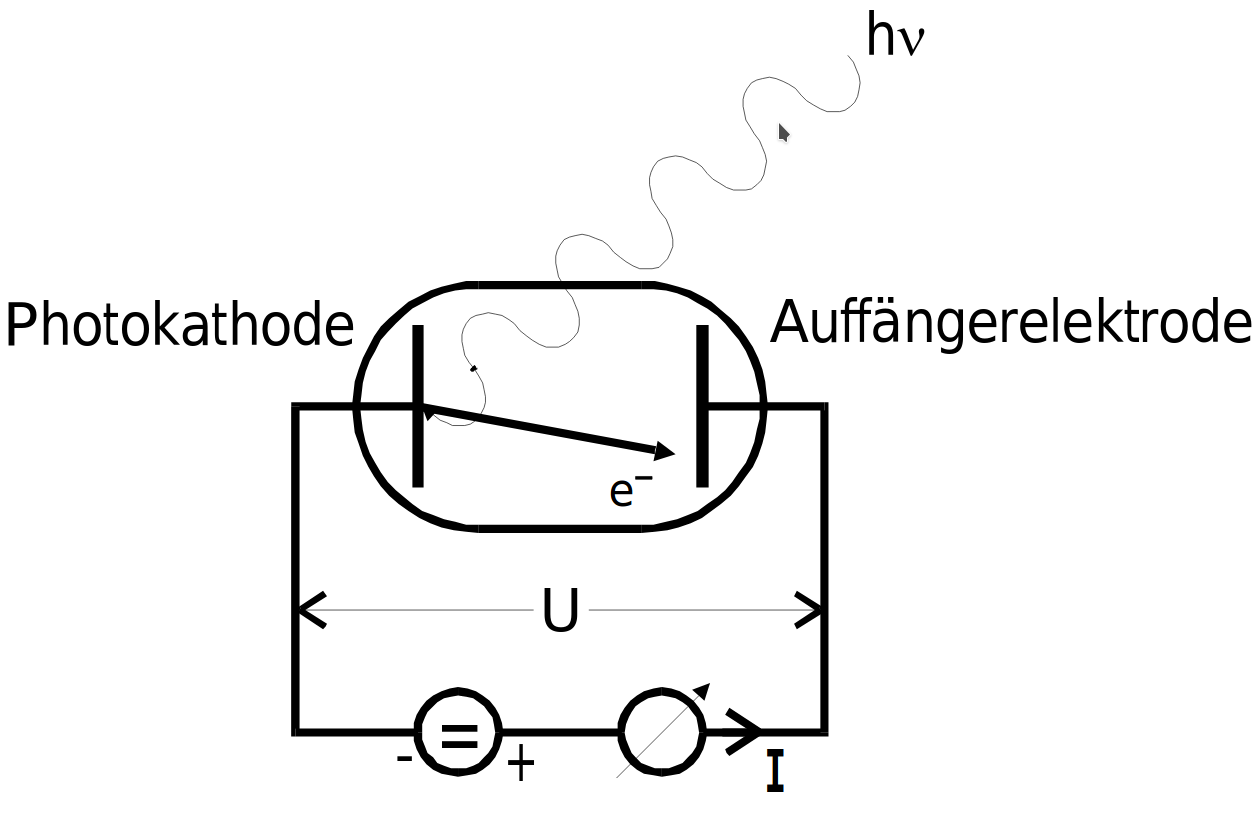
\includegraphics[width=0.5\textwidth]{content/data/aufbau.png}
    \caption{Der prinzipielle Auffbau für die Untersuchung des Photoeffekts. Grafik entnommen aus Versuchsanleitung \cite{anleitung}.}
    \label{fig:aufbau}
\end{figure}

Ein prinzipieller Aufbau ist in Abbildung \ref{fig:aufbau} zu sehen.
Es ist zu erkennen, dass auf einer der Platten das Licht der Engerie $\nu h$ trifft.
Zwischen den PLatten wird eine Spannung angelegt, diese ist frei regulierbar.
Wenn nun eine Spannung angelegt wird, die gerade so groß ist, dass die Elektronen aus dem Metall gelöst werden, aber nicht die andere Platte erreichen, kann durch
\begin{equation}
eU = \frac{1}{2} m_\text{e} v^2
\label{eq:grenzenergie}
\end{equation}
die Energie der Elektronen berechnet werden.
$U$ entspricht dabei der angelegten Spannung, $e$ der elementar Ladung, $m$ der Masse des Elektrons und $v$ der Geschwindigkeit, der schnellesten Elektronen.
Es ist allerdings schwierig diese Granzspannung zuverlässig zu bestimmen, da nicht alle Elektronen die selbe Energie besitzten.
Die Energie der Elektronen entspricht viel mehr einer Verteilung von $0$ bis $\frac{1}{2}mv^2$, da die Elektronen bereits im Festkörper eine Enrgie besitzten.
Daher wird zur Berechung der Grenzspannung $U_\text{G}$, die Wurzel des Stroms $\sqrt{I}$ zwischen den beiden Platten gegen die angelegte Spannung $U$ aufgetragen.
Da teilweise mit recht Energie armen Licht gearbeitet wird, wird bei diesem eine Beschleunigungsspannung ansatt einer Bremsspannung genutzt.